\newpage

\section{Предложенный метод и его корректность}
Опираясь на оригинальную статью LoRA~\cite{hu2021lora}, в этой работе LoRA была применина к задаче классификации. Структура LoRA адаптера:
\begin{center}
\begin{tabular}{ | c | c| } 
 \hline
  Fine tuning & LoRA fine tuning\\ 
 \hline
 $W_{upd} = W + \Delta W$ & $W_{upd} = W + AB$\\ 
 $\hat{y} = xW_{upd}= x(W + \Delta W)$ & $\hat{y} = xW_{upd}= x(W + AB)$\\
 $\hat{y} = xW + x\Delta W$ & $\hat{y} = xW + xAB$ \\
 \hline
\end{tabular}
\end{center}
Где $W \in \mathbb{R}^{d \times k}$ - предобученные веса, $\Delta W \in \mathbb{R}^{d \times k}$ - матрица обновленных весов. $\Delta W$ is приближается с помощью метода LoRA произведением $A \cdot B$, где $A \in \mathbb{R}^{d \times r}$, $B \in \mathbb{R}^{r \times k}$ и $r$ - гиперпараметр ранга. \newline
Здесь $A \sim \mathcal{N}(0,\,\sigma^{2})$ и $B = [0]_{r \times k}$.


\textit{Докажем состоятельность предложенной модели}\\
Сходимость традиционной модели трансформер была доказана в работе~\cite{lee2023mathematical}. Доказательство приведено для задачи классификации:

\subsection{Теорема 1~\cite{lee2023mathematical}}
\begin{theorem}
Будем считать, что: 
\begin{itemize}
    \item Существует модель с набором параметров $\theta^*$, которая может аппроксимировать достоверное распределение, сгенерированное данными, с минимальным расхождением по KL-дивергенции: 
    \begin{equation}
    \label{eq:1}
    \exists \theta^*: \theta^* = \argmin _\theta D_{KL}(P_{true} \mid\mid P_{model}(\cdot, \theta))
    \end{equation}
     \item По мере увеличения размера набора данных $\hat{V}$ эмпирическое распределение приближается к истинному распределению, генерирующему данные.
     \item $\mathscr{L}(\theta)$ - непрерывная, дифференцируемая. Где
\end{itemize} 
\begin{equation}
\label{eq:2}
\mathscr{L}(\theta) = -\sum_{X_i \in \hat{V} \subset V^{*}} \sum_{c_i \in [N_c]} \log \left(P_{\Phi_0+\Delta \Phi(\theta)}\left(c_i \mid X_i\right)\right)
\end{equation}

Тогда минимизация $\mathscr{L}(\theta)$ приводит к получению оценки истинного распределения, генерирующего данные.

\end{theorem}
\renewcommand\qedsymbol{$\blacksquare$}
\begin{proof}
Докажем сходимость следующей функции:

Согласно минимизации функции эмпирического риска, минимум $\mathscr{L}(\theta)$ приближается к минимуму матожидания риска, поскольку размер $\hat{V}$ стремится к бесконечности.
\begin{equation}
\label{eq:3}
\begin{aligned}
\lim_{\mid\hat{V}\mid\to\infty} \argmin _\theta \E \mathscr{L}(\theta) =\\
\argmin _\theta \E _{X_i\in P_{true}}[\sum_{c_i \in [N_c]} \log \left(P_{\Phi_0+\Delta \Phi(\theta)}\left(c_i \mid X_i\right)\right] =\\
\argmin _\theta D_{KL}(P_{true}\mid\mid P_{model}(\theta)) = \theta^*
\end{aligned}
\end{equation}

Равенство~\eqref{eq:3} верно в силу равномерной сходимости $\mathscr{L}(\theta)$ и в силу определения KL-дивергенции.
\begin{equation}
\label{eq:4}
D_{KL}(P || Q)=\int_{-\infty}^{\infty} p(x) \log \left(\frac{p(x)}{q(x)}\right) dx = \E _{x \sim p(x)}[\log \left(\frac{p(x)}{q(x)}\right)]
\end{equation}
\end{proof}

 Докажем, что LoRA применима к задаче классификации. LoRA  используется для решения различных проблем seq2seq, таких как:\\~\cite{zhang2023adding},~\cite{dettmers2024qlora},~\cite{dai2024instructblip}. Этот подход особенно популярен в задачах преобразования видео в текст, так как им(задачам) свойственны "богатые распределения входных данных и разнообразие задач, обусловленные дополнительным визуальным входным данным"~\cite{dai2024instructblip}. 

В то же время для решения задачи классификации с помощью BERT~\cite{vaswani2017attention} требуется не более чем дополнительный softmax слой после BERT~\cite{sun2019fine}: 
\begin{equation}
\label{eq:5}
\begin{aligned}
p(c \mid \mathbf{x})=\operatorname{softmax}(W^T \mathbf{x})\\
\hat{\mathbf{y}}=\operatorname{softmax}\left(W^T \mathbf{x}\right)=\frac{\exp \left(W^T \mathbf{x}\right)}{\sum_{i=1}^k \exp \left(W^T \mathbf{x}\right)_i}
\end{aligned}
\end{equation}
Где $\mathbf{x}$ - это выходной результат последнего слоя BERT.\\
Структура BERT:

\begin{figure}[h]
    \centering
    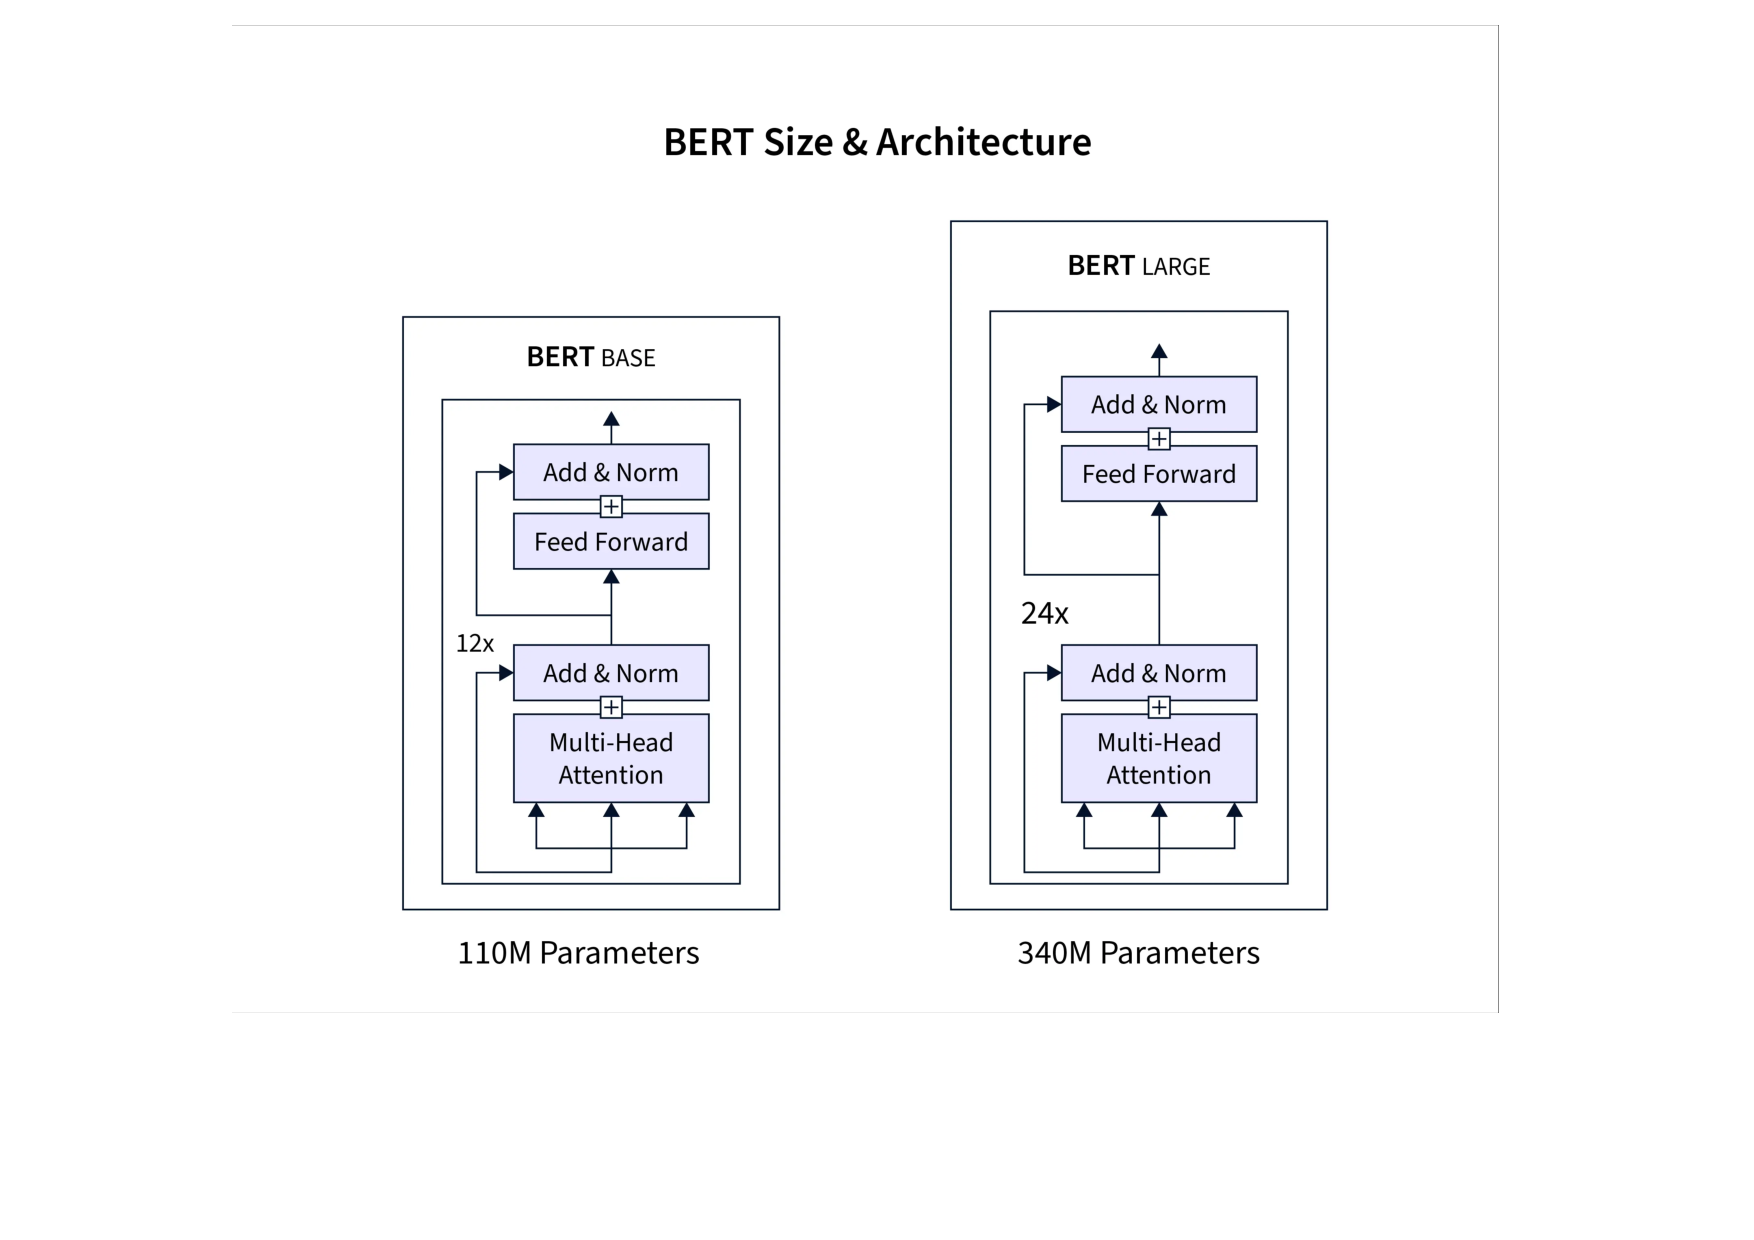
\includegraphics[width=1.0\textwidth]{images/bert_architecture copy.pdf}
    \caption{BERT structure}
\end{figure}

\newpage
Где, согласно~\cite{thickstun2021transformer},\\
Attention:
\begin{equation}
\begin{aligned}
Q^{(h)}\left(\mathbf{x}_i\right)=W_{h, q}^T \mathbf{x}_i, \quad K^{(h)}\left(\mathbf{x}_i\right)=W_{h, k}^T \mathbf{x}_i, \\ V^{(h)}\left(\mathbf{x}_i\right)=W_{h, v}^T \mathbf{x}_i, \quad W_{h, q}, W_{h, k}, W_{h, v} \in \mathbb{R}^{d \times k} 
\end{aligned}
\end{equation}
\begin{equation}
\begin{aligned}
\alpha_{i,j}^{(h)}=\operatorname{softmax}_j\left(\frac{\left\langle Q^{(h)}\left(\mathbf{x}_i\right), K^{(h)}\left(\mathbf{x}_j\right)\right\rangle}{\sqrt{k}}\right), \\
\mathbf{u}_i^{\prime}=\sum_{h=1}^H W_{c, h}^T \sum_{j=1}^n \alpha_{i, j}^{(h)} V^{(h)}\left(\mathbf{x}_j\right), \\
\end{aligned}
\end{equation}
LayerNorm,
Feed Forward Network,
LayerNorm:
\begin{equation}
\begin{aligned}
&\mathbf{u}_i=\operatorname{LayerNorm}\left(\mathbf{x}_i+\mathbf{u}_i^{\prime} ; \gamma_1, \beta_1\right), \\
& \mathbf{z}_i^{\prime}=W_2^T \operatorname{ReLU}\left(W_1^T \mathbf{u}_i\right), \\
& \mathbf{z}_i=\text { LayerNorm }\left(\mathbf{u}_i+\mathbf{z}_i^{\prime} ; \gamma_2, \beta_2\right) \text {, }
\end{aligned}
\end{equation}
Layer normalization может быть переписана в соответствии с оригинальной статьей~\cite{ba2016layer}:
\begin{equation}
\begin{aligned}
& \operatorname{LayerNorm}(\mathbf{z} ; \gamma, \beta)=\gamma \frac{\left(\mathbf{z}-\mu_{\mathbf{z}}\right)}{\sigma_{\mathbf{z}}}+\beta, \\
& \gamma, \beta \in \mathbb{R}^k . \\
& \mu_{\mathbf{z}}=\frac{1}{k} \sum_{i=1}^k \mathbf{z}_i, \quad \sigma_{\mathbf{z}}=\sqrt{\frac{1}{k} \sum_{i=1}^k\left(\mathbf{z}_i-\mu_{\mathbf{z}}\right)^2} . \\
&
\end{aligned}
\end{equation}

\subsection{Теорема 2}
\begin{theorem}
В рамках задачи классификации, при заданных условиях:
\begin{itemize}
    \item Модель семейства Bert с указанной выше математической структурой и дополнительным слоем 
    \begin{equation}
    \label{eq:6}
        \hat{\mathbf{y}}=\operatorname{softmax}\left(W_{upd}^T \mathbf{x}\right)=\frac{\exp \left(W_{upd}^T \mathbf{x}\right)}{\sum_{i=1}^k \exp \left(W_{upd}^T \mathbf{x}\right)_i}
    \end{equation}
    где 
    \begin{equation}
    \label{eq:7}
    W_{upd} =\underset{(d \times k) }{W} + \underset{(d \times k)}{\Delta W}
    \end{equation}
    и $x$ - это выходной результат BERT, $W$ - матрица весов, $\Delta W$ - матрица обновленных весов.
    \item  Данная модель Bert без дополнительного слоя также корректно работает с аппроксимацией 
    \begin{equation}
    \label{eq:8}
    \underset{(d \times k)}{\Delta W} = \underset{(d \times r)}{ A} \times \underset{(r \times k)}{B}
    \end{equation}
    \item Выполняется lemma 1.0.1. (можно считать данную модель состоятельной).
\end{itemize}
Тогда можно утверждать, что при~\eqref{eq:10} заданная модель BERT с дополнительным слоем гарантирует корректную выходную матрицу.
\end{theorem}
\renewcommand\qedsymbol{$\blacksquare$}
\begin{proof} 
Докажем, что выход из дополнительного слоя корректен:\\ По дистрибутивному свойству сложения матриц и ассоциативному свойтсву произведения матриц: 
\begin{equation}
\label{eq:9}
\begin{aligned}
\hat{\mathbf{y}} = \operatorname{softmax}\left(W_{upd}^T \mathbf{x}\right) =
\operatorname{softmax}\left((W + \Delta W)^T \mathbf{x}\right) =\\ \\
= \frac{\exp \left(W^T \mathbf{x} + \Delta W^T \mathbf{x}\right)}{\sum_{i=1}^k \exp \left(W^T \mathbf{x} + \Delta W^T \mathbf{x}\right)_i}=\\ \\
= \frac{\exp \left(W^T \mathbf{x}\right) \exp \left(\Delta W^T \mathbf{x}\right)}{\sum_{i=1}^k \exp \left(W^T \mathbf{x}\right)_i \exp \left(\Delta W^T \mathbf{x}\right)_i}
\end{aligned}
\end{equation} 
где $\mathbf{x}$ - выходная матрица последнего слоя Bert.
$\mathbf{x}$ корректна по условию.\\
В предложенной модели с использованием LoRA:
\begin{equation}
\label{eq:10}
\begin{aligned}
\hat{\mathbf{y}} = \operatorname{softmax}\left(W_{upd} \mathbf{x}\right) =
\operatorname{softmax}\left((W + AB)^T \mathbf{x}\right) =\\ \\
= \frac{\exp \left(W^T \mathbf{x} + (AB)^T \mathbf{x}\right)}{\sum_{i=1}^k \exp \left(W^T \mathbf{x} + (AB)^T \mathbf{x}\right)_i}=\\ \\
= \frac{\exp \left(W^T \mathbf{x}\right) \exp \left((AB)^T \mathbf{x}\right)}{\sum_{i=1}^k \exp \left(W^T \mathbf{x}\right)_i \exp \left((AB)^T \mathbf{x}\right)_i}
\end{aligned}
\end{equation} 
где $\mathbf{x}$ также выходная матрица BERT с LoRA и $\mathbf{x}$ корректна по условию. \newline
Так как финальные размерности остались неизменными, как и $W^T\mathbf{x}$, легко заметить: 
\begin{equation}
\label{eq:11}
\begin{aligned}
 \underset{(k \times d)}{\Delta W^T} \times \mathbf{x} = u\\
(\underset{(d \times r)}{A} \times \underset{(r \times k)}{B})^T \times \mathbf{x} = (\underset{(k \times r)}{B^T} \times \underset{(r \times d)}{A^T}) \times \mathbf{x} = u^*
\end{aligned}
\end{equation}
Так как~\eqref{eq:10}, можно заключить что ${u^*} = {u}$ и является корретной матрицей, а следовательно предложенная модель работает корректно.
\end{proof}
